\documentclass[11pt]{article}\usepackage[]{graphicx}\usepackage[]{color}
%% maxwidth is the original width if it is less than linewidth
%% otherwise use linewidth (to make sure the graphics do not exceed the margin)
\makeatletter
\def\maxwidth{ %
  \ifdim\Gin@nat@width>\linewidth
    \linewidth
  \else
    \Gin@nat@width
  \fi
}
\makeatother

\definecolor{fgcolor}{rgb}{0.345, 0.345, 0.345}
\newcommand{\hlnum}[1]{\textcolor[rgb]{0.686,0.059,0.569}{#1}}%
\newcommand{\hlstr}[1]{\textcolor[rgb]{0.192,0.494,0.8}{#1}}%
\newcommand{\hlcom}[1]{\textcolor[rgb]{0.678,0.584,0.686}{\textit{#1}}}%
\newcommand{\hlopt}[1]{\textcolor[rgb]{0,0,0}{#1}}%
\newcommand{\hlstd}[1]{\textcolor[rgb]{0.345,0.345,0.345}{#1}}%
\newcommand{\hlkwa}[1]{\textcolor[rgb]{0.161,0.373,0.58}{\textbf{#1}}}%
\newcommand{\hlkwb}[1]{\textcolor[rgb]{0.69,0.353,0.396}{#1}}%
\newcommand{\hlkwc}[1]{\textcolor[rgb]{0.333,0.667,0.333}{#1}}%
\newcommand{\hlkwd}[1]{\textcolor[rgb]{0.737,0.353,0.396}{\textbf{#1}}}%
\let\hlipl\hlkwb

\usepackage{framed}
\makeatletter
\newenvironment{kframe}{%
 \def\at@end@of@kframe{}%
 \ifinner\ifhmode%
  \def\at@end@of@kframe{\end{minipage}}%
  \begin{minipage}{\columnwidth}%
 \fi\fi%
 \def\FrameCommand##1{\hskip\@totalleftmargin \hskip-\fboxsep
 \colorbox{shadecolor}{##1}\hskip-\fboxsep
     % There is no \\@totalrightmargin, so:
     \hskip-\linewidth \hskip-\@totalleftmargin \hskip\columnwidth}%
 \MakeFramed {\advance\hsize-\width
   \@totalleftmargin\z@ \linewidth\hsize
   \@setminipage}}%
 {\par\unskip\endMakeFramed%
 \at@end@of@kframe}
\makeatother

\definecolor{shadecolor}{rgb}{.97, .97, .97}
\definecolor{messagecolor}{rgb}{0, 0, 0}
\definecolor{warningcolor}{rgb}{1, 0, 1}
\definecolor{errorcolor}{rgb}{1, 0, 0}
\newenvironment{knitrout}{}{} % an empty environment to be redefined in TeX

\usepackage{alltt}

\usepackage{hyperref, lastpage, fancyhdr,multicol,caption,subcaption,tabularx}
\usepackage{amsmath,graphicx}
\usepackage{float}

\usepackage{geometry}
\usepackage{pdflscape}



\topmargin      -1.5cm   % read Lamport p.163
\oddsidemargin  -0.04cm  % read Lamport p.163
\evensidemargin -0.04cm  % same as oddsidemargin but for left-hand pages
\textwidth      16.59cm
\textheight     23.94cm
\parskip         7.2pt   % sets spacing between paragraphs
\parindent         0pt   % sets leading space for paragraphs
\pagestyle{empty}        % Uncomment if don't want page numbers
\pagestyle{fancyplain}

\usepackage{natbib} %need this for bibtex
\IfFileExists{upquote.sty}{\usepackage{upquote}}{}

\lhead{}
\chead{}
\rhead{}

\usepackage{setspace} %for double spacing
\doublespacing
\IfFileExists{upquote.sty}{\usepackage{upquote}}{}
\begin{document}




\begin{knitrout}
\definecolor{shadecolor}{rgb}{0.969, 0.969, 0.969}\color{fgcolor}\begin{kframe}
\begin{alltt}
\hlkwd{sum}\hlstd{(nhanes}\hlopt{$}\hlstd{modvigmin}\hlopt{==}\hlnum{0}\hlstd{)}\hlopt{/}\hlkwd{nrow}\hlstd{(nhanes)}
\end{alltt}
\begin{verbatim}
## [1] 0.07841659
\end{verbatim}
\begin{alltt}
\hlkwd{sum}\hlstd{(nhanes}\hlopt{$}\hlstd{vigmin}\hlopt{==}\hlnum{0}\hlstd{)}\hlopt{/}\hlkwd{nrow}\hlstd{(nhanes)}
\end{alltt}
\begin{verbatim}
## [1] 0.8801602
\end{verbatim}
\begin{alltt}
\hlkwd{sum}\hlstd{(nhanes}\hlopt{$}\hlstd{lightmin}\hlopt{==}\hlnum{0}\hlstd{)}\hlopt{/}\hlkwd{nrow}\hlstd{(nhanes)}
\end{alltt}
\begin{verbatim}
## [1] 0
\end{verbatim}
\end{kframe}
\end{knitrout}

\begin{knitrout}
\definecolor{shadecolor}{rgb}{0.969, 0.969, 0.969}\color{fgcolor}\begin{kframe}
\begin{alltt}
\hlcom{#no diff in modmin by day really except 7th}
\hlstd{nhanes} \hlopt \hlkwd{group_by}\hlstd{(rep)} \hlopt \hlkwd{summarise}\hlstd{(}\hlkwc{m}\hlstd{=}\hlkwd{mean}\hlstd{(modvigmin),}\hlkwc{s}\hlstd{=}\hlkwd{sd}\hlstd{(modmin)}\hlopt{/}\hlkwd{sqrt}\hlstd{(}\hlkwd{length}\hlstd{(modmin)))}
\end{alltt}
\begin{verbatim}
## # A tibble: 7 � 3
##     rep        m         s
##   <int>    <dbl>     <dbl>
## 1     1 22.60066 0.3411052
## 2     2 23.01777 0.3518468
## 3     3 22.96771 0.3583861
## 4     4 22.41386 0.3488521
## 5     5 22.24356 0.3589189
## 6     6 21.15523 0.3571320
## 7     7 19.41996 0.3616865
\end{verbatim}
\begin{alltt}
\hlcom{#no diff in modmin by day really except 7th and 2nd}
\hlstd{nhanes} \hlopt \hlkwd{group_by}\hlstd{(rep)} \hlopt \hlkwd{summarise}\hlstd{(}\hlkwc{m}\hlstd{=}\hlkwd{mean}\hlstd{(lightmin),}\hlkwc{s}\hlstd{=}\hlkwd{sd}\hlstd{(lightmin)}\hlopt{/}\hlkwd{sqrt}\hlstd{(}\hlkwd{length}\hlstd{(lightmin)))}
\end{alltt}
\begin{verbatim}
## # A tibble: 7 � 3
##     rep        m        s
##   <int>    <dbl>    <dbl>
## 1     1 258.6827 1.048918
## 2     2 261.5339 1.093391
## 3     3 258.6147 1.096388
## 4     4 258.8213 1.136550
## 5     5 258.2212 1.160056
## 6     6 255.2295 1.186014
## 7     7 244.4119 1.253172
\end{verbatim}
\begin{alltt}
\hlcom{#mondays most vig, fri-sun least, tues-thurs similar}
\hlstd{nhanes} \hlopt \hlkwd{group_by}\hlstd{(rep)} \hlopt \hlkwd{summarise}\hlstd{(}\hlkwc{m}\hlstd{=}\hlkwd{mean}\hlstd{(vigmin),}\hlkwc{s}\hlstd{=}\hlkwd{sd}\hlstd{(vigmin)}\hlopt{/}\hlkwd{sqrt}\hlstd{(}\hlkwd{length}\hlstd{(lightmin)))}
\end{alltt}
\begin{verbatim}
## # A tibble: 7 � 3
##     rep         m          s
##   <int>     <dbl>      <dbl>
## 1     1 0.9411853 0.06110670
## 2     2 0.8115414 0.05276647
## 3     3 0.8965840 0.06021138
## 4     4 0.7660865 0.05689883
## 5     5 0.7392597 0.05397894
## 6     6 0.8310108 0.06361269
## 7     7 0.6902050 0.06106663
\end{verbatim}
\begin{alltt}
\hlkwd{anova}\hlstd{(}\hlkwd{lm}\hlstd{(modvigmin}\hlopt{~}\hlkwd{as.factor}\hlstd{(rep),}\hlkwc{data}\hlstd{=}\hlkwd{subset}\hlstd{(nhanes,rep}\hlopt{<}\hlnum{6}\hlstd{)))} \hlcom{#first 5 days are similar, last two}
\end{alltt}
\begin{verbatim}
## Analysis of Variance Table
## 
## Response: modvigmin
##                   Df   Sum Sq Mean Sq F value Pr(>F)
## as.factor(rep)     4     2902  725.44  0.8288 0.5065
## Residuals      31937 27954416  875.30
\end{verbatim}
\end{kframe}
\end{knitrout}

\begin{knitrout}
\definecolor{shadecolor}{rgb}{0.969, 0.969, 0.969}\color{fgcolor}\begin{kframe}
\begin{alltt}
\hlcom{#weekends lower}
\hlstd{nhanes} \hlopt \hlkwd{group_by}\hlstd{(dow)} \hlopt \hlkwd{summarise}\hlstd{(}\hlkwc{m}\hlstd{=}\hlkwd{mean}\hlstd{(modvigmin),}\hlkwc{s}\hlstd{=}\hlkwd{sd}\hlstd{(modvigmin)}\hlopt{/}\hlkwd{sqrt}\hlstd{(}\hlkwd{length}\hlstd{(modvigmin)))}
\end{alltt}
\begin{verbatim}
## # A tibble: 7 � 3
##     dow        m         s
##   <int>    <dbl>     <dbl>
## 1     1 17.46672 0.3539009
## 2     2 23.63394 0.3753241
## 3     3 23.49455 0.3683897
## 4     4 23.63173 0.3842220
## 5     5 23.18340 0.3712310
## 6     6 22.43408 0.3639320
## 7     7 19.52794 0.3799264
\end{verbatim}
\begin{alltt}
\hlcom{#weekends and thursday lower, friday higher}
\hlstd{nhanes} \hlopt \hlkwd{group_by}\hlstd{(dow)} \hlopt \hlkwd{summarise}\hlstd{(}\hlkwc{m}\hlstd{=}\hlkwd{mean}\hlstd{(lightmin),}\hlkwc{s}\hlstd{=}\hlkwd{sd}\hlstd{(lightmin)}\hlopt{/}\hlkwd{sqrt}\hlstd{(}\hlkwd{length}\hlstd{(lightmin)))}
\end{alltt}
\begin{verbatim}
## # A tibble: 7 � 3
##     dow        m        s
##   <int>    <dbl>    <dbl>
## 1     1 239.7397 1.171315
## 2     2 259.8399 1.106457
## 3     3 260.0095 1.095333
## 4     4 259.8370 1.102353
## 5     5 256.6507 1.103868
## 6     6 263.0100 1.146749
## 7     7 256.8055 1.218114
\end{verbatim}
\begin{alltt}
\hlcom{#first day vig}
\hlstd{nhanes} \hlopt \hlkwd{group_by}\hlstd{(dow)} \hlopt \hlkwd{summarise}\hlstd{(}\hlkwc{m}\hlstd{=}\hlkwd{mean}\hlstd{(vigmin),}\hlkwc{s}\hlstd{=}\hlkwd{sd}\hlstd{(vigmin)}\hlopt{/}\hlkwd{sqrt}\hlstd{(}\hlkwd{length}\hlstd{(lightmin)))}
\end{alltt}
\begin{verbatim}
## # A tibble: 7 � 3
##     dow         m          s
##   <int>     <dbl>      <dbl>
## 1     1 0.7239862 0.06502960
## 2     2 0.9462687 0.06184397
## 3     3 0.8742129 0.05357820
## 4     4 0.8859250 0.06278267
## 5     5 0.8446359 0.05683506
## 6     6 0.7264334 0.05487292
## 7     7 0.6707994 0.05419137
\end{verbatim}
\begin{alltt}
\hlkwd{anova}\hlstd{(}\hlkwd{lm}\hlstd{(modvigmin}\hlopt{~}\hlkwd{as.factor}\hlstd{(dow),}\hlkwc{data}\hlstd{=}\hlkwd{subset}\hlstd{(nhanes,dow}\hlopt\hlkwd{c}\hlstd{(}\hlnum{2}\hlopt{:}\hlnum{6}\hlstd{))))} \hlcom{#M-F similar}
\end{alltt}
\begin{verbatim}
## Analysis of Variance Table
## 
## Response: modvigmin
##                   Df   Sum Sq Mean Sq F value Pr(>F)
## as.factor(dow)     4     6363 1590.75  1.7992 0.1259
## Residuals      31803 28118692  884.15
\end{verbatim}
\end{kframe}
\end{knitrout}


\begin{knitrout}
\definecolor{shadecolor}{rgb}{0.969, 0.969, 0.969}\color{fgcolor}\begin{kframe}
\begin{alltt}
\hlcom{#test for weekend effects}
\hlkwd{anova}\hlstd{(}\hlkwd{lm}\hlstd{(modvigmin} \hlopt{~} \hlkwd{as.factor}\hlstd{(weekend),}\hlkwc{data}\hlstd{=nhanes))}
\end{alltt}
\begin{verbatim}
## Analysis of Variance Table
## 
## Response: modvigmin
##                       Df   Sum Sq Mean Sq F value    Pr(>F)    
## as.factor(weekend)     1   181096  181096  214.83 < 2.2e-16 ***
## Residuals          42438 35773439     843                      
## ---
## Signif. codes:  0 '***' 0.001 '**' 0.01 '*' 0.05 '.' 0.1 ' ' 1
\end{verbatim}
\begin{alltt}
\hlkwd{anova}\hlstd{(}\hlkwd{lm}\hlstd{(lightmin} \hlopt{~} \hlkwd{as.factor}\hlstd{(weekend),}\hlkwc{data}\hlstd{=nhanes))}
\end{alltt}
\begin{verbatim}
## Analysis of Variance Table
## 
## Response: lightmin
##                       Df    Sum Sq Mean Sq F value    Pr(>F)    
## as.factor(weekend)     1   1042016 1042016  133.48 < 2.2e-16 ***
## Residuals          42438 331295573    7807                      
## ---
## Signif. codes:  0 '***' 0.001 '**' 0.01 '*' 0.05 '.' 0.1 ' ' 1
\end{verbatim}
\begin{alltt}
\hlkwd{anova}\hlstd{(}\hlkwd{lm}\hlstd{(vigmin} \hlopt{~} \hlkwd{as.factor}\hlstd{(weekend),}\hlkwc{data}\hlstd{=nhanes))}
\end{alltt}
\begin{verbatim}
## Analysis of Variance Table
## 
## Response: vigmin
##                       Df Sum Sq Mean Sq F value  Pr(>F)   
## as.factor(weekend)     1    202 202.477   9.714 0.00183 **
## Residuals          42438 884572  20.844                   
## ---
## Signif. codes:  0 '***' 0.001 '**' 0.01 '*' 0.05 '.' 0.1 ' ' 1
\end{verbatim}
\end{kframe}
\end{knitrout}

\begin{knitrout}
\definecolor{shadecolor}{rgb}{0.969, 0.969, 0.969}\color{fgcolor}\begin{kframe}
\begin{alltt}
\hlstd{nrep} \hlkwb{<-} \hlstd{(nhanes} \hlopt \hlkwd{group_by}\hlstd{(id)} \hlopt \hlkwd{summarise}\hlstd{(}\hlkwc{n}\hlstd{=}\hlkwd{length}\hlstd{(id)))}\hlopt{$}\hlstd{n}

\hlcom{#m1 <- lme(modvigmin~1,data=nhanes,random=~1|id,correlation=corAR1(form=~1|id),method="ML")}
\hlstd{m1} \hlkwb{<-} \hlkwd{lme}\hlstd{(modvigmin}\hlopt{~}\hlkwd{as.factor}\hlstd{(rep)}\hlopt{+}\hlkwd{as.factor}\hlstd{(dow),}\hlkwc{data}\hlstd{=nhanes,}\hlkwc{random}\hlstd{=}\hlopt{~}\hlnum{1}\hlopt{|}\hlstd{id,}\hlkwc{method}\hlstd{=}\hlstr{"ML"}\hlstd{)}

\hlstd{re} \hlkwb{<-} \hlkwd{rep}\hlstd{(}\hlkwd{unlist}\hlstd{(}\hlkwd{ranef}\hlstd{(m1)),nrep)}
\hlstd{nhanes}\hlopt{$}\hlstd{error} \hlkwb{<-} \hlstd{nhanes}\hlopt{$}\hlstd{modvigmin}  \hlopt{-} \hlkwd{predict}\hlstd{(m1)}
\hlstd{eht} \hlkwb{<-} \hlstd{nhanes} \hlopt \hlkwd{group_by}\hlstd{(id)} \hlopt \hlkwd{summarise}\hlstd{(}\hlkwc{e1}\hlstd{=error[}\hlnum{1}\hlstd{],}\hlkwc{e2}\hlstd{=error[}\hlnum{2}\hlstd{],}\hlkwc{e3}\hlstd{=error[}\hlnum{3}\hlstd{],}\hlkwc{e4}\hlstd{=error[}\hlnum{4}\hlstd{],}\hlkwc{e5}\hlstd{=error[}\hlnum{5}\hlstd{],}\hlkwc{e6}\hlstd{=error[}\hlnum{6}\hlstd{],}\hlkwc{e7}\hlstd{=error[}\hlnum{7}\hlstd{])}

\hlcom{# ind <- which(!is.na(eht$e7))}
\hlcom{# boxtest <- rep(0,length(ind))}
\hlcom{# for(i in 1:length(ind))\{}
\hlcom{#   boxtest[i] <- Box.test(unlist(eht[ind[i],-1]),lag=2,type="Ljung-Box")$p.value}
\hlcom{# \}}
\hlcom{# summary(boxtest)}

\hlcom{#lag 1 difference}
\hlstd{o1a} \hlkwb{=} \hlkwd{c}\hlstd{(eht}\hlopt{$}\hlstd{e1[nrep} \hlopt{>} \hlnum{1}\hlstd{],eht}\hlopt{$}\hlstd{e2[nrep} \hlopt{>} \hlnum{2}\hlstd{],eht}\hlopt{$}\hlstd{e3[nrep} \hlopt{>} \hlnum{3}\hlstd{],eht}\hlopt{$}\hlstd{e4[nrep} \hlopt{>} \hlnum{4}\hlstd{],eht}\hlopt{$}\hlstd{e5[nrep} \hlopt{>} \hlnum{5}\hlstd{],eht}\hlopt{$}\hlstd{e6[nrep} \hlopt{>} \hlnum{6}\hlstd{])}
\hlstd{o1b} \hlkwb{=} \hlkwd{c}\hlstd{(eht}\hlopt{$}\hlstd{e2[nrep} \hlopt{>} \hlnum{1}\hlstd{],eht}\hlopt{$}\hlstd{e3[nrep} \hlopt{>} \hlnum{2}\hlstd{],eht}\hlopt{$}\hlstd{e4[nrep} \hlopt{>} \hlnum{3}\hlstd{],eht}\hlopt{$}\hlstd{e5[nrep} \hlopt{>} \hlnum{4}\hlstd{],eht}\hlopt{$}\hlstd{e6[nrep} \hlopt{>} \hlnum{5}\hlstd{],eht}\hlopt{$}\hlstd{e7[nrep} \hlopt{>} \hlnum{6}\hlstd{])}
\hlkwd{cor}\hlstd{(o1a,o1b)}
\end{alltt}
\begin{verbatim}
## [1] -0.1000537
\end{verbatim}
\begin{alltt}
\hlcom{#lag 2 diff}
\hlstd{o2a} \hlkwb{=} \hlkwd{c}\hlstd{(eht}\hlopt{$}\hlstd{e1[nrep} \hlopt{>} \hlnum{2}\hlstd{],eht}\hlopt{$}\hlstd{e2[nrep} \hlopt{>} \hlnum{3}\hlstd{],eht}\hlopt{$}\hlstd{e3[nrep} \hlopt{>} \hlnum{4}\hlstd{],eht}\hlopt{$}\hlstd{e4[nrep} \hlopt{>} \hlnum{5}\hlstd{],eht}\hlopt{$}\hlstd{e5[nrep} \hlopt{>} \hlnum{6}\hlstd{])}
\hlstd{o2b} \hlkwb{=} \hlkwd{c}\hlstd{(eht}\hlopt{$}\hlstd{e3[nrep} \hlopt{>} \hlnum{2}\hlstd{],eht}\hlopt{$}\hlstd{e4[nrep} \hlopt{>} \hlnum{3}\hlstd{],eht}\hlopt{$}\hlstd{e5[nrep} \hlopt{>} \hlnum{4}\hlstd{],eht}\hlopt{$}\hlstd{e6[nrep} \hlopt{>} \hlnum{5}\hlstd{],eht}\hlopt{$}\hlstd{e7[nrep} \hlopt{>} \hlnum{6}\hlstd{])}
\hlkwd{cor}\hlstd{(o2a,o2b)}
\end{alltt}
\begin{verbatim}
## [1] -0.1892647
\end{verbatim}
\begin{alltt}
\hlcom{#lag 3 diff  }
\hlstd{o3a} \hlkwb{=} \hlkwd{c}\hlstd{(eht}\hlopt{$}\hlstd{e1[nrep} \hlopt{>} \hlnum{3}\hlstd{],eht}\hlopt{$}\hlstd{e2[nrep} \hlopt{>} \hlnum{4}\hlstd{],eht}\hlopt{$}\hlstd{e3[nrep} \hlopt{>} \hlnum{5}\hlstd{],eht}\hlopt{$}\hlstd{e4[nrep} \hlopt{>} \hlnum{6}\hlstd{])}
\hlstd{o3b} \hlkwb{=} \hlkwd{c}\hlstd{(eht}\hlopt{$}\hlstd{e4[nrep} \hlopt{>} \hlnum{3}\hlstd{],eht}\hlopt{$}\hlstd{e5[nrep} \hlopt{>} \hlnum{4}\hlstd{],eht}\hlopt{$}\hlstd{e6[nrep} \hlopt{>} \hlnum{5}\hlstd{],eht}\hlopt{$}\hlstd{e7[nrep} \hlopt{>} \hlnum{6}\hlstd{])}
\hlkwd{cor}\hlstd{(o3a,o3b)}
\end{alltt}
\begin{verbatim}
## [1] -0.2558842
\end{verbatim}
\begin{alltt}
\hlcom{#lag 4 diff}
\hlstd{o4a} \hlkwb{=} \hlkwd{c}\hlstd{(eht}\hlopt{$}\hlstd{e1[nrep} \hlopt{>} \hlnum{4}\hlstd{],eht}\hlopt{$}\hlstd{e2[nrep} \hlopt{>} \hlnum{5}\hlstd{],eht}\hlopt{$}\hlstd{e3[nrep} \hlopt{>} \hlnum{6}\hlstd{])}
\hlstd{o4b} \hlkwb{=} \hlkwd{c}\hlstd{(eht}\hlopt{$}\hlstd{e5[nrep} \hlopt{>} \hlnum{4}\hlstd{],eht}\hlopt{$}\hlstd{e6[nrep} \hlopt{>} \hlnum{5}\hlstd{],eht}\hlopt{$}\hlstd{e7[nrep} \hlopt{>} \hlnum{6}\hlstd{])}
\hlkwd{cor}\hlstd{(o4a,o4b)}
\end{alltt}
\begin{verbatim}
## [1] -0.2653008
\end{verbatim}
\begin{alltt}
\hlcom{#lag 5 diff}
\hlstd{o5a} \hlkwb{=} \hlkwd{c}\hlstd{(eht}\hlopt{$}\hlstd{e1[nrep} \hlopt{>} \hlnum{5}\hlstd{],eht}\hlopt{$}\hlstd{e2[nrep} \hlopt{>} \hlnum{6}\hlstd{])}
\hlstd{o5b} \hlkwb{=} \hlkwd{c}\hlstd{(eht}\hlopt{$}\hlstd{e6[nrep} \hlopt{>} \hlnum{5}\hlstd{],eht}\hlopt{$}\hlstd{e7[nrep} \hlopt{>} \hlnum{6}\hlstd{])}
\hlkwd{cor}\hlstd{(o5a,o5b)}
\end{alltt}
\begin{verbatim}
## [1] -0.1862721
\end{verbatim}
\end{kframe}
\end{knitrout}


\begin{knitrout}
\definecolor{shadecolor}{rgb}{0.969, 0.969, 0.969}\color{fgcolor}
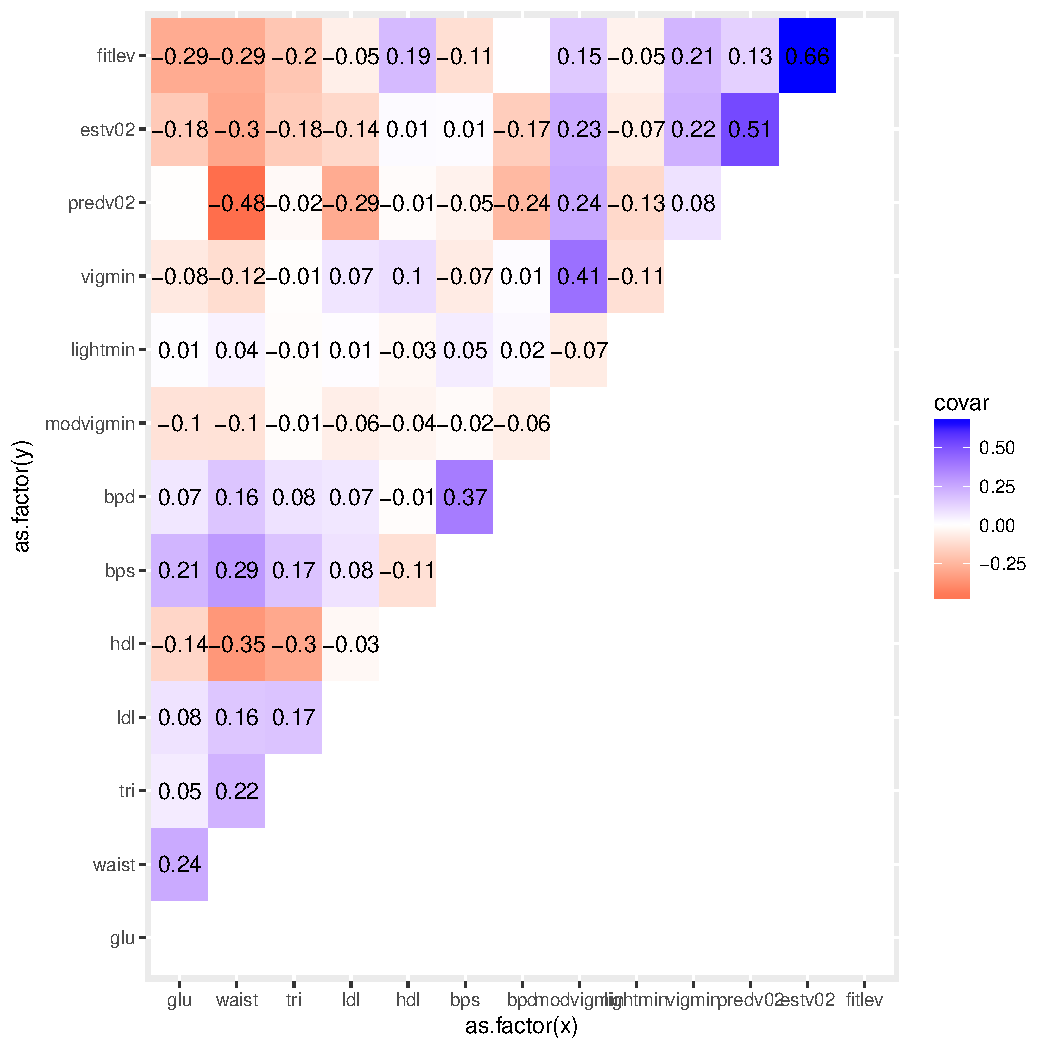
\includegraphics[width=\maxwidth]{figure/c7-1} 

\end{knitrout}


\begin{knitrout}
\definecolor{shadecolor}{rgb}{0.969, 0.969, 0.969}\color{fgcolor}\begin{kframe}
\begin{alltt}
\hlcom{#multivariate regression on mean observed modvig, light}
\hlstd{a} \hlkwb{<-} \hlstd{nhanes} \hlopt \hlkwd{group_by}\hlstd{(id)} \hlopt \hlkwd{summarise}\hlstd{(}\hlkwc{modvig}\hlstd{=}\hlkwd{mean}\hlstd{(modvigmin),}\hlkwc{light}\hlstd{=}\hlkwd{mean}\hlstd{(lightmin))}
\hlstd{y}\hlopt{$}\hlstd{modvig} \hlkwb{<-} \hlstd{a}\hlopt{$}\hlstd{modvig}
\hlstd{y}\hlopt{$}\hlstd{light} \hlkwb{<-} \hlstd{a}\hlopt{$}\hlstd{light}

\hlstd{m3} \hlkwb{<-} \hlkwd{lm}\hlstd{(}\hlkwd{with}\hlstd{(y,}\hlkwd{cbind}\hlstd{(glu,waist,tri,hdl,bps,bpd))}\hlopt{~}\hlstd{y}\hlopt{$}\hlstd{modvig)}
\hlkwd{summary}\hlstd{(m3)}
\end{alltt}
\begin{verbatim}
## Response glu :
## 
## Call:
## lm(formula = glu ~ y$modvig)
## 
## Residuals:
##    Min     1Q Median     3Q    Max 
## -62.50 -14.31  -6.71   2.63 440.78 
## 
## Coefficients:
##              Estimate Std. Error t value Pr(>|t|)    
## (Intercept) 107.87227    0.74640 144.524   <2e-16 ***
## y$modvig     -0.18519    0.02181  -8.491   <2e-16 ***
## ---
## Signif. codes:  0 '***' 0.001 '**' 0.01 '*' 0.05 '.' 0.1 ' ' 1
## 
## Residual standard error: 32.92 on 3574 degrees of freedom
##   (4668 observations deleted due to missingness)
## Multiple R-squared:  0.01977,	Adjusted R-squared:  0.0195 
## F-statistic:  72.1 on 1 and 3574 DF,  p-value: < 2.2e-16
## 
## 
## Response waist :
## 
## Call:
## lm(formula = waist ~ y$modvig)
## 
## Residuals:
##     Min      1Q  Median      3Q     Max 
## -37.507 -10.795  -1.156   9.475  58.162 
## 
## Coefficients:
##              Estimate Std. Error t value Pr(>|t|)    
## (Intercept) 100.19115    0.34288  292.20   <2e-16 ***
## y$modvig     -0.12379    0.01002  -12.36   <2e-16 ***
## ---
## Signif. codes:  0 '***' 0.001 '**' 0.01 '*' 0.05 '.' 0.1 ' ' 1
## 
## Residual standard error: 15.12 on 3574 degrees of freedom
##   (4668 observations deleted due to missingness)
## Multiple R-squared:  0.04096,	Adjusted R-squared:  0.0407 
## F-statistic: 152.7 on 1 and 3574 DF,  p-value: < 2.2e-16
## 
## 
## Response tri :
## 
## Call:
## lm(formula = tri ~ y$modvig)
## 
## Residuals:
##     Min      1Q  Median      3Q     Max 
## -121.18  -65.00  -30.59   27.40 2585.85 
## 
## Coefficients:
##              Estimate Std. Error t value Pr(>|t|)    
## (Intercept) 154.32305    2.85134  54.123  < 2e-16 ***
## y$modvig     -0.40685    0.08331  -4.883 1.09e-06 ***
## ---
## Signif. codes:  0 '***' 0.001 '**' 0.01 '*' 0.05 '.' 0.1 ' ' 1
## 
## Residual standard error: 125.7 on 3574 degrees of freedom
##   (4668 observations deleted due to missingness)
## Multiple R-squared:  0.006628,	Adjusted R-squared:  0.00635 
## F-statistic: 23.85 on 1 and 3574 DF,  p-value: 1.089e-06
## 
## 
## Response hdl :
## 
## Call:
## lm(formula = hdl ~ y$modvig)
## 
## Residuals:
##     Min      1Q  Median      3Q     Max 
## -38.675 -11.922  -2.698   9.320 132.359 
## 
## Coefficients:
##             Estimate Std. Error t value Pr(>|t|)    
## (Intercept)  55.6949     0.3695 150.740   <2e-16 ***
## y$modvig     -0.0233     0.0108  -2.158    0.031 *  
## ---
## Signif. codes:  0 '***' 0.001 '**' 0.01 '*' 0.05 '.' 0.1 ' ' 1
## 
## Residual standard error: 16.29 on 3574 degrees of freedom
##   (4668 observations deleted due to missingness)
## Multiple R-squared:  0.001302,	Adjusted R-squared:  0.001022 
## F-statistic: 4.658 on 1 and 3574 DF,  p-value: 0.03097
## 
## 
## Response bps :
## 
## Call:
## lm(formula = bps ~ y$modvig)
## 
## Residuals:
##     Min      1Q  Median      3Q     Max 
## -44.510 -13.122  -2.921  10.172  93.694 
## 
## Coefficients:
##              Estimate Std. Error t value Pr(>|t|)    
## (Intercept) 126.33975    0.43377  291.26   <2e-16 ***
## y$modvig     -0.13340    0.01267  -10.53   <2e-16 ***
## ---
## Signif. codes:  0 '***' 0.001 '**' 0.01 '*' 0.05 '.' 0.1 ' ' 1
## 
## Residual standard error: 19.13 on 3574 degrees of freedom
##   (4668 observations deleted due to missingness)
## Multiple R-squared:  0.03006,	Adjusted R-squared:  0.02979 
## F-statistic: 110.8 on 1 and 3574 DF,  p-value: < 2.2e-16
## 
## 
## Response bpd :
## 
## Call:
## lm(formula = bpd ~ y$modvig)
## 
## Residuals:
##     Min      1Q  Median      3Q     Max 
## -68.064  -7.423   0.529   8.164  47.533 
## 
## Coefficients:
##              Estimate Std. Error t value Pr(>|t|)    
## (Intercept) 67.729506   0.310267 218.294   <2e-16 ***
## y$modvig     0.013836   0.009066   1.526    0.127    
## ---
## Signif. codes:  0 '***' 0.001 '**' 0.01 '*' 0.05 '.' 0.1 ' ' 1
## 
## Residual standard error: 13.68 on 3574 degrees of freedom
##   (4668 observations deleted due to missingness)
## Multiple R-squared:  0.0006513,	Adjusted R-squared:  0.0003717 
## F-statistic: 2.329 on 1 and 3574 DF,  p-value: 0.1271
\end{verbatim}
\end{kframe}
\end{knitrout}

\begin{knitrout}
\definecolor{shadecolor}{rgb}{0.969, 0.969, 0.969}\color{fgcolor}\begin{kframe}


{\ttfamily\noindent\itshape\color{messagecolor}{\#\# Using\ \ as id variables}}

{\ttfamily\noindent\itshape\color{messagecolor}{\#\# `stat\_bin()` using `bins = 30`. Pick better value with `binwidth`.}}

{\ttfamily\noindent\color{warningcolor}{\#\# Warning: Removed 14799 rows containing non-finite values (stat\_bin).}}\end{kframe}
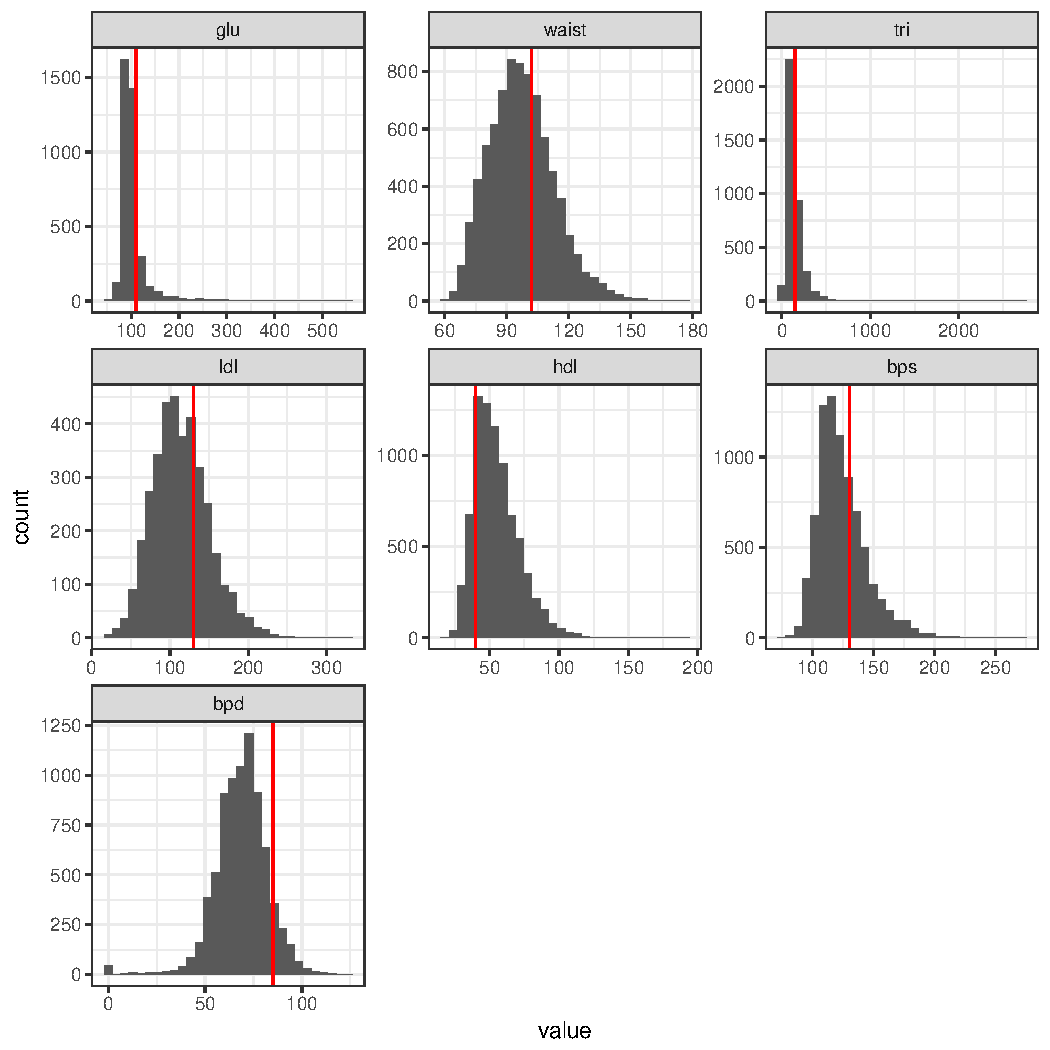
\includegraphics[width=\maxwidth]{figure/c9-1} 

\end{knitrout}

\begin{knitrout}
\definecolor{shadecolor}{rgb}{0.969, 0.969, 0.969}\color{fgcolor}\begin{kframe}


{\ttfamily\noindent\itshape\color{messagecolor}{\#\# `stat\_bin()` using `bins = 30`. Pick better value with `binwidth`.\\\#\# `stat\_bin()` using `bins = 30`. Pick better value with `binwidth`.\\\#\# `stat\_bin()` using `bins = 30`. Pick better value with `binwidth`.}}\end{kframe}
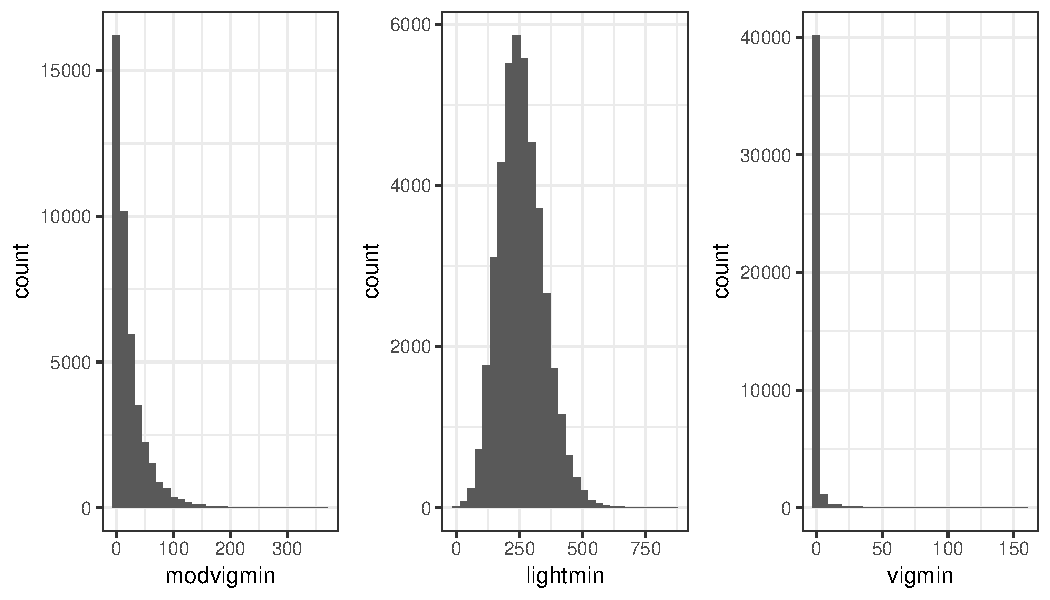
\includegraphics[width=\maxwidth]{figure/c10-1} 

\end{knitrout}


\end{document}
